This sub section relates to
the ``LSTM network'' block in Fig. \ref{fi:overall}.

In our work, we represent a video as $n$
fixed-length segments ($n$ differ for videos of different lengths),  with overlapping frames.  Each segment
is represented with a fused vector $c_{t}$. Therefore, each video can be represented as a vector time series.


Now, each vector time series could be  analyzed using traditional time series modeling techniques,
such as Auto Regressive Moving Average, to obtain features or model parameters, to describe the
vector time series.
But the main drawback of these methods is that they model current values of a series as a function of past values
and have finite dynamic response to time series input. Also they lack the ability to grasp the internal state
representations of a complex time series. RNNs maintain hidden layers with directed feedback connections, and hence,
have an infinite dynamic response. While training, it learns internal states of a sequence
and are usually performed better in modeling complex dynamic temporal patterns of long sequences.


However, it is not ideal to train standard RNNs to solve problems,
which require learning of long-term temporal dependencies. This is because of the vanishing-gradient problem, which occurs
due to the exponential decay of gradient loss of the function with respect to time.

In practice, LSTM networks typically perform better in such cases.
LSTM networks are a special type of RNN, which include a ``memory cell'', and as the name suggests,
it can maintain a certain state, in memory, for longer periods of time.
It also has a set of control gates for controlling the removal or addition information to the cell state.
This special architecture gives them the ability to capture longer-term dependencies. First, we revise the operation of a LSTM
network.

The most important structure of a LSTM unit is its memory cell $c_{t}$, which preserves the state. Basic structure of a LSTM
unit is shown in figure. The memory cell is self connected, and it has three gates(multiplicative units), i.e., input gate, forget gate and
output gate, which are used to control, how much to store, remove or output long range contextual information of a temporal sequence.

The detailed activation process of the memory cell and three gates, as shown in Fig. \ref{fi:lstmblock} are
illustrated as follows:


\begin{figure}
  \centering
  \begin{tikzpicture}[x=0.5cm, y=0.5cm, every node/.append style={text=black, font=\scriptsize}]

	\node [draw, circle, minimum height=18, fill=blue!20] (input) at (0,0) {$i^t$};
	\node [draw, circle, minimum height=18, fill=blue!20] (output) at (6,0) {$o^t$};	
	\node [draw, circle, minimum height=18, fill=red!20] (a) at (-2,-2) {};	
	\node [draw, circle, minimum height=8] (b) at (0,-2) {};
	\node [draw, circle, minimum height=24, fill=green!20] (c) at (2,-2) {$c^t$};	
	\node [draw, circle, minimum height=18, fill=red!20] (d) at (4,-2) {};	
	\node [draw, circle, minimum height=8] (e) at (6,-2) {};	
	\node [] (h) at (8,-2) {$h^t$};	
	\node [draw, circle, minimum height=8] (g) at (2,-3.5) {};	
	\node [draw, circle, minimum height=18, fill=blue!20] (f) at (2,-5) {$f^t$};		
	
	\draw (a.south west) .. controls ( $(a) +(0.2,-0.4)$)  and  ( $(a) +(-0.2,0.4)$) .. (a.north east);
	\draw (d.south west) .. controls ( $(d) +(0.2,-0.4)$)  and  ( $(d) +(-0.2,0.4)$) .. (d.north east);
	\draw (b.south west) -- (b.north east) (b.north west) -- (b.south east);
	\draw (e.south west) -- (e.north east) (e.north west) -- (e.south east);
	\draw (g.south west) -- (g.north east) (g.north west) -- (g.south east);	
	
	\draw[-latex] (a) -- (b);
	\draw[-latex] (b) -- (c);
	\draw[-latex] (c) -- (d);
	\draw[-latex] (d) -- (e);
	\draw[-latex] (e) -- (h);
	\draw[-latex] (output) -- (e);
	\draw[-latex] (c) -- (output);
	\draw[-latex] (c) -- (input);
	\draw[-latex] (input) -- (b);
	\draw[-latex] (f) -- (g);
	
	\draw[-latex] (c)  to[out=-150,in=-180] 	(f);
	
	\draw[-latex] (c.south east)   to[out=-45,in=0] 	node[midway, anchor=west] {Feedback} (g.east) ;
	\draw[-latex] (g.west)   to[out=180,in=-135] 	(c.south west);	
	
	\draw[latex-] (input) -- ++(60:1.5);
	\draw[latex-] (input) -- ++(90:1.5) node[anchor=south] {$X^t$};
	\draw[latex-] (input) -- ++(120:1.5);
	
	\draw[latex-] (output) -- ++(60:1.5);
	\draw[latex-] (output) -- ++(90:1.5) node[anchor=south] {$X^t$};
	\draw[latex-] (output) -- ++(120:1.5);	
	
	
	\draw[latex-] (a) -- ++(150:1.5);
	\draw[latex-] (a) -- ++(180:1.5) node[anchor=east] {$X^t$};;
	\draw[latex-] (a) -- ++(210:1.5);
	
	\draw[latex-] (f) -- ++(-120:1.5);
	\draw[latex-] (f) -- ++(-90:1.5) node[anchor=north] {$X^t$};;
	\draw[latex-] (f) -- ++(-60:1.5);
	
	\node at (f.east) [anchor=west] {Forget gate};
	\node at (output.west) [anchor=east, text width=0.8cm] {Output gate};
	\node at (input.west) [anchor=east, text width=0.6cm] {Input gate};
	\node at (c.north) [anchor=south] {Cell};

\draw  (-2.8,0.9) rectangle (7,-6);
\end{tikzpicture}
  \caption{Long short-term memory (LSTM) block cell. Source XX.}\label{fi:lstmblock}
\end{figure}

\begin{equation}
i^{t} = \sigma (W_{xi}x^t + W_{hi}h^{t-1} + W_{ci}c^{t-1} + b_{i})
\end{equation}
\begin{equation}
f^{t} = \sigma (W_{xf}x^t + W_{hf}h^{t-1} + W_{cf}c^{t-1} + b_{f})
\end{equation}
\begin{equation}
c^{t} = f^tc^{t-1} + i^ttanh(W_{xc}x^t + W_{hc}h^{t-1} + b_{c})
\end{equation}
\begin{equation}
o^{t} = \sigma (W_{xo}x^t + W_{ho}h^{t-1} + W_{co}c^{t-1} + b_{o})
\end{equation}
\begin{equation}
h^t = o^t\tanh(c^t)
\end{equation}

Where $W$ is the connection weight between two units and $\sigma(\cdot)$ is the sigmoid function.

Since the LSTM network is used only for capturing the temporal dynamic patterns between sub actions, one LSTM layer is enough.
Our LSTM network is shown in figure \ref{fi:layers}. The network consists of an input layer, a 128 unit LSTM layer with 0.8 dropout, and
a fully connected softmax output layer. As we have a sequence of activities per one classification, we use many to one approach,
for feeding the fusioned vectors to the network, as shown in figure \ref{fi:lstm}

\begin{figure}
  \centering
  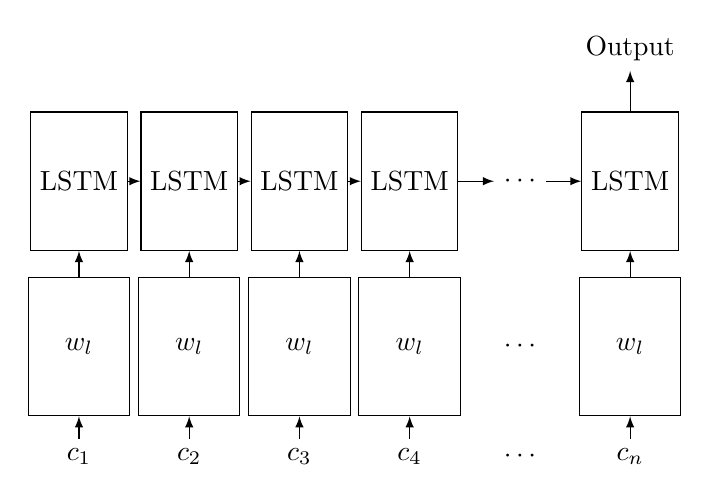
\begin{tikzpicture}[x=0.7cm, y=0.7cm] 
	\foreach \i/\l in {1/1, 2/2, 3/3, 4/4, 6/n}
	{
		\node[draw=black, minimum height=50] (1\i) at (2*\i, 0) {LSTM};
		\node[draw=black, minimum height=50, text width=30, align=center] (2\i) at (2*\i, -3) {$w_l$};
		\node[text width=30, align=center] (3\i) at (2*\i, -5) {$c_\l$};		
	}
	
	\node (15) at (2*5,0) {$\cdots$};
	\node (25) at (2*5,-3) {$\cdots$};
	\node (35) at (2*5,-5) {$\cdots$};	
	
	\foreach  \i/\j in {1/2, 2/3, 3/4, 4/5, 5/6}
	{
		\draw [-latex] (1\i) -- (1\j);
	}
	
	\foreach  \i in {1,2,3,4,6}
	{
		\draw [-latex] (2\i) -- (1\i);
		\draw [-latex] (3\i) -- (2\i);
	}	
	
	\draw[-latex] (16) -- +(0,2) node [anchor=south] {Output};
	

\end{tikzpicture}
  \caption{The process of feeding fused vectors to the LSTM network. $c_{i}$ indicates the fused vector representing the $i_{th}$
  video segment.}\label{fi:lstm}
\end{figure}

\begin{figure}
  \centering
  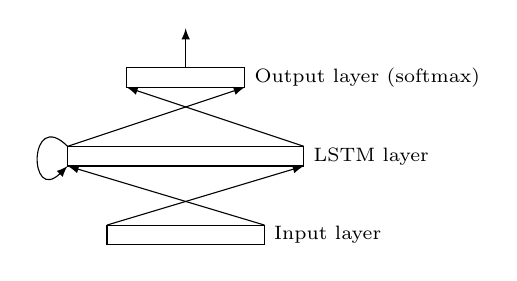
\begin{tikzpicture}[x=0.5cm, y=0.5cm, every node/.append style={text=black, font=\scriptsize}]
	\draw  (0,0) -- ++(2, 0) -- ++(0, 0.5) coordinate  (a)  node [midway, anchor=west] {Input layer} -- ++(-4, 0) coordinate  (b) -- ++(0, -0.5) -- cycle;
	
	
	\draw  (0,2) -- ++(3, 0) coordinate  (c) -- ++(0, 0.5) coordinate (d) node [midway, anchor=west] {LSTM layer}  -- ++(-6, 0) coordinate  (e) -- ++(0, -0.5)  coordinate  (f)  -- cycle;
	
	\draw  (0,4) -- ++(1.5, 0)  coordinate  (g) -- ++(0, 0.5) node [midway, anchor=west] {Output layer (softmax)}  -- ++(-3, 0) coordinate[midway] (t) -- ++(0, -0.5) coordinate  (h) -- cycle;	
	
	\draw[-latex] (a) -- (f);
	\draw[-latex] (b) -- (c);
	
	\draw[-latex] (e) -- (g);
	\draw[-latex] (d) -- (h);	
	
	\draw[-latex] (t) -- ++(0, 1);		
	\draw[-latex] (e)  .. controls ++(-1,1) and ++(-1, -1) ..  (f);
\end{tikzpicture}
  \caption{A simple illustration of the LSTM network. The network consists of an input layer, a 128 unit LSTM layer with 0.8 dropout, and
a fully connected softmax output layer.}\label{fi:layers}
\end{figure}

